\section{Архитектура библиотеки}

В данной секции предлагается рассмотреть архитектуру разрабатываемой библиотеки, ее основные компоненты и модули, а также последовательность обработки операций на GPU. Библиотека спроектирована с учетом основных аспектов, связанных с осуществлением вычислений на GPU, рассмотренных в предыдущей главе.

Структура библиотеки и ее конченная функциональность определяется следующими высокоуровневыми требованиями, которые продиктованы конечными вычислительными задачами и особенностями реализации существующих решений.

\begin{itemize}%[noitemsep,topsep=0pt,parsep=0pt,partopsep=0pt]
    \item \textbf{Использование OpenCL API.} Библиотека должна использовать OpenCL API для ускорения вычислений на одном или нескольких OpenCL-совместимых GPU-устройств в системе. Данный API поддерживается на множестве графических ускорителей, а также позволяет динамически во время исполнения компилировать GPU-код, что избавляет пользователя от установки и использования стороннего специализированного компилятора.
    
    \item \textbf{Пользовательские типы данных.} Библиотека предоставляет возможность для создания произвольных пользовательских типов. Тип представляется уникальным именем и размером элементов в байтах. Элементы типа являются POD-структурами, обрабатываются как обычные последовательности байтов. 
    
    \item \textbf{Пользовательские функции.} Библиотека предоставляет возможность создания пользовательских функций, которые могут принимать на вход пользовательские (произвольные) типы, и которые могут быть использованы чтобы параметризовать математические операции. Функции определяются в виде набора сток с OpenCL-кодом, что позволяет создавать функции без использования сторонних инструментов для компиляции пользовательского кода. 
    
    \item \textbf{Граф выражений.} Пользователь определяет задачи для вычислений в виде ориентированного ациклического графа выражений, используя интерфейс библиотеки для создания узлов графа и зависимостей между узлами в декларативном стиле. Затем пользователь передает весь граф библиотеке для выполнения, и может в блокирующем и неблокирующем режиме получить результат.
    
    \item \textbf{Автоматическое распределение вычислений.} Библиотека автоматически выполняет разбиение графа выражений на множество задач и подзадач, которые упорядочиваются в соответствии с зависимостями и распределяются между всеми доступными GPU-устройствами вычислителя. Данная работа скрыта от пользователя и не требует от него действий. 
   
    \item \textbf{Автоматическое распределение данных}. Библиотека автоматически выполняет форматирование данных, хранит их в гибридном формате и автоматически распределяет между вычислительными узлами.  Данная работа, формат хранения, детали распределения скрыты от пользователя и не требует от него действий.
\end{itemize}

\begin{figure}[h]
    \centering
    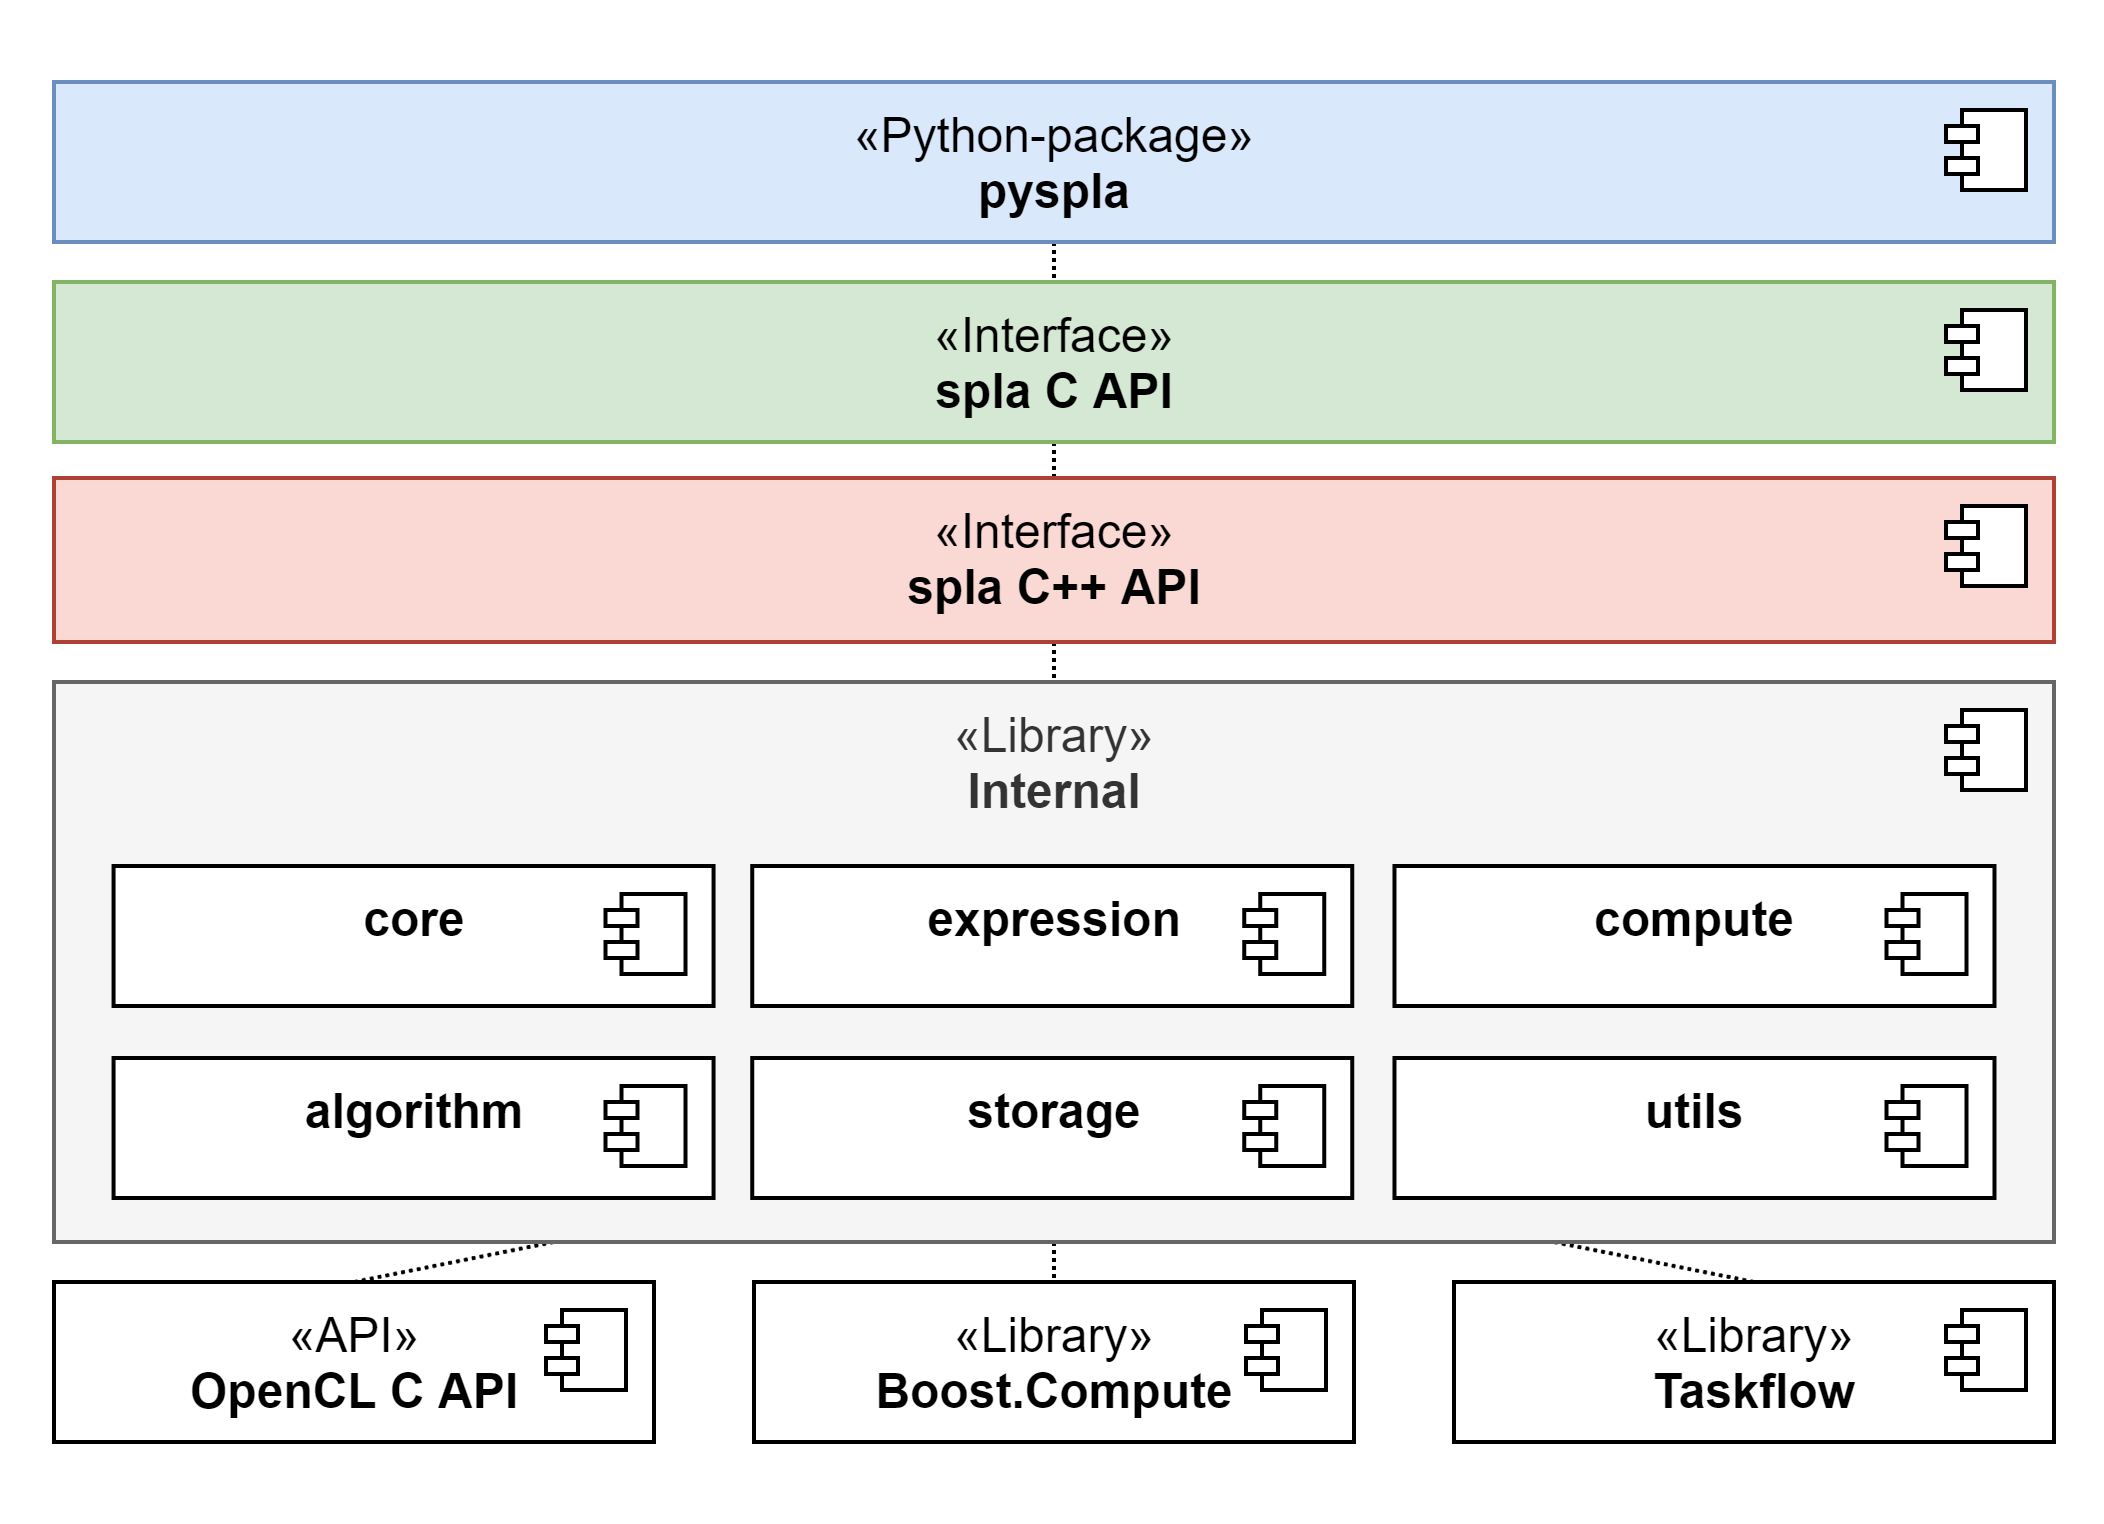
\includegraphics[width=0.7\textwidth]{images/spla_architecture.png}
    \caption{Архитектура библиотеки}
    \label{fig:spla_architecture}
\end{figure}

\subsection{Компоненты библиотеки}

Далее предлагается рассмотреть высокоуровневую структуру разрабатываемой библиотеки \textit{spla}. Диаграмма основных компонентов представлена на рисунке~\ref{fig:spla_architecture}. В данной диаграмме зависимости между компонентами направленны сверху вниз, модули расположены внутри одной компоненты имеют общий уровень в иерархии. Детальное описание отдельных частей диаграммы представлено ниже.

\begin{itemize}
    \item Pyspla --- это Python-пакет для работы с примитивами библиотеки в высокоуровной среде языка Python. Данный пакет предназначен для конечных пользователей. Он будет предоставлять средства для прототипирования и запуска алгоритмов, а также будет расширять функциональность исходной библиотеки за счет введения дополнительных операций и за счет синтаксического сахара, доступного в языке Python.
    
    \item Spla C API --- это C99 совместимы интерфейс библиотеки для ее использования в С-приложения. Данный интерфейс требуется как для экспортирования методов и операций в Python-пакет за счет методов вызова функций из скомпилированной библиотеки с разделяемым кодом, так и для написания высокопроизводительных прикладных алгоритмах с минимальным количеством накладных расходов.
    
    \item Spla C++ API --- основной интерфейс библиотеки. Предоставляет доступ ко всем примитивам и операциям библиотеки. Интерфейс не использует шаблоны. Для автоматизации управления временем жизни объектов используется встроенный механизма подсчета ссылок на объекты, что позволяет их передавать в любые вычислительные выражения.
    
    \item Intenral --- детали реализации библиотеки, полностью скрытые для внешнего пользователя. Далее предлагается кратко рассмотреть основные модули реализации:
    
    \begin{itemize}
        \item Core --- ядро библиотеки. Поддерживает глобальное состояние, предоставляет доступ ко всем вспомогательным и основным подсистемам библиотеки. 
        \item Storage --- предоставляет средства для автоматизированного гибридного хранения матриц и векторов. Матрицы и вектора хранятся в виде двумерной или одномерной сетки блоков. Каждый блок имеет свой собственный формат хранения.
        \item Expression --- механизм для трансляции входных графов выражений в ациклический граф задач, который можно выполнить на множестве потоков процессора. 
        \item Algorithm --- модуль, который хранит множетсво алгоритмов для обработки блоков матриц и векторов в разных форматах и разных сочетаниях.
        \item Compute --- вспомогательные базовые алгоритмы, расширяющие функциональность библиотеки Boost.Compute.
        \item Utils --- утилиты, используемые в библиотеке.
    \end{itemize}
    
    \item Сторонние зависимости. Для работы с GPU-устройством используется OpenCL API. Boost.Compute~\cite{article:boost_compute} является надстройкой над OpenCL. Он предоставляет реализацию базовых алгоритмов (\textit{sort}, \textit{scatter}, и т.д.) и контейнеров для данных (\textit{vector}, \textit{iterator}) для вычислений на GPU-устройстве. Taskflow~\cite{article:taskflow} используется в качестве многопоточного менеджера задач, который позволяет выполнять пользовательские задачи в виде ориентированного графа с зависимостями. 
\end{itemize}